\documentclass[12pt]{article}
\usepackage[utf8]{inputenc}
\usepackage{fullpage}
\usepackage[top=2cm, bottom=4cm, left=2cm, right=2cm]{geometry}
\usepackage{amsmath,amsthm,amsfonts,amssymb,amscd}
\usepackage{lastpage}
\usepackage{enumerate}
\usepackage{fancyhdr}
\usepackage{mathrsfs}
\usepackage[dvipsnames]{xcolor}
\usepackage{graphicx}
\usepackage{listings}
\usepackage{hyperref}
\usepackage{titlesec}
\usepackage{bm}
\usepackage[ruled]{algorithm2e}

\usepackage{fancyvrb}

\newtheorem{definition}{Definition}
\newtheorem{theorem}{Theorem}[section]
\newtheorem{corollary}{Corollary}
\newtheorem{notation}{Notation}
\newtheorem{remark}{Remark}
\newtheorem{claim}{Claim}
\newtheorem{fact}{Fact}
\newtheorem{facts}{Facts}

\newcommand{\Data}{\mathcal{D}}
\newcommand{\Exmt}{\mathcal{E}}
\newcommand{\Expect}{\mathbb{E}}
\newcommand{\ErrIn}{E_{\text{in}}}
\newcommand{\ErrOut}{E_{\text{out}}}
\newcommand{\ApxErrOut}{E_{\text{test}}}
\newcommand{\Bias}{\bm{\mathrm{bias}}}
\newcommand{\Var}{\bm{\mathrm{var}}}

\newcommand{\myvec}[1]{\mathbf{#1}}
\newcommand{\X}{\myvec{x}}

\newcommand{\gD}{g^{(\Data)}}
\def\beloweq#1#2{\underset{\displaystyle\overset{\displaystyle\shortparallel}{#2}}{#1}}

% change vertical spacing for align
\setlength{\jot}{2ex}

%%%%%%% taken from overleaf example %%%%%%%

%New colors defined below
\definecolor{codegreen}{rgb}{0,0.6,0}
\definecolor{codegray}{rgb}{0.5,0.5,0.5}
\definecolor{codepurple}{rgb}{0.58,0,0.82}
\definecolor{backcolour}{rgb}{0.95,0.95,0.92}

%Code listing style named "mystyle"
\lstdefinestyle{mystyle}{
  backgroundcolor=\color{backcolour},   commentstyle=\color{codegreen},
  keywordstyle=\color{magenta},
  numberstyle=\tiny\color{codegray},
  stringstyle=\color{codepurple},
  basicstyle=\ttfamily\footnotesize,
  breakatwhitespace=false,         
  breaklines=true,                 
  captionpos=b,                    
  keepspaces=true,                 
  numbers=left,                    
  numbersep=5pt,                  
  showspaces=false,                
  showstringspaces=false,
  showtabs=false,                  
  tabsize=2
}
\lstdefinestyle{mystyle_top}{
  backgroundcolor=\color{backcolour},   commentstyle=\color{codegreen},
  keywordstyle=\color{magenta},
  numberstyle=\tiny\color{codegray},
  stringstyle=\color{codepurple},
  basicstyle=\ttfamily\footnotesize,
  breakatwhitespace=false,         
  breaklines=true,                 
  captionpos=t,                    
  keepspaces=true,                 
  numbers=left,                    
  numbersep=5pt,                  
  showspaces=false,                
  showstringspaces=false,
  showtabs=false,                  
  tabsize=2
}
%"mystyle" code listing set
\lstset{style=mystyle}


%%%%%%% taken from overleaf example %%%%%%%

%%%%%%% taken from https://tex.stackexchange.com/questions/85200/include-data-from-a-txt-verbatim example %%%%%%%
% redefine \VerbatimInput
\RecustomVerbatimCommand{\VerbatimInput}{VerbatimInput}%
{fontsize=\footnotesize,
 %
 frame=lines,  % top and bottom rule only
 framesep=2em, % separation between frame and text
 rulecolor=\color{Gray},
 %
 label=\fbox{\color{Black}label},
 labelposition=topline,
 %
 commandchars=\|\(\), % escape character and argument delimiters for
                      % commands within the verbatim
%  commentchar=*        % comment character
}
%%%%%%% taken from https://tex.stackexchange.com/questions/85200/include-data-from-a-txt-verbatim example %%%%%%%

%%%%
\pagestyle{fancyplain}
\setcounter{MaxMatrixCols}{20}

\titleformat{\section}
  {\normalfont\scshape}{\thesection}{1em}{}

\setlength{\parindent}{0.0in}
\setlength{\parskip}{0.05in}


\headheight 25pt
\lhead{Jamie Lea}
\chead{CS 5340 Machine Learning}
\rhead{Project 4}

\headsep 1.5em

\usepackage[style=ACM-Reference-Format,backend=bibtex,sorting=none]{biblatex}

\addbibresource{aml_bib.bib} %Imports bibliography file

\begin{document}

What follows is my submission for Project 4 in Machine Learning.  The goal was to answer Problem 2.24 in \textit{Learning From Data}.\cite{AML:LFD}   

\section*{Problem 2.24\cite{AML:LFD}}

Consider a simplified learning scenario.  Assume that the input dimension is one.  Assume that the input variable $x$ is uniformly distributed in the interval $[-1, 1]$.  The data consists of 2 points $\{x_{1}, x_{2}\}$ and assume that the target function is $f(x) = x^{2}$.  Thus, the full data set is $\Data = \{(x_{1}, x_{1}^{2}), (x_{2}, x_{2}^{2})\}$.  The learning algorithm returns the line fitting these two points as $g$ ($\mathcal{H}$ consists of functions of the form $h(x) = ax + b$).  We are interested in the test performance ($\Expect[\ErrOut])$ of our learning system with respect to the squared error measure, the $\Bias$ and the $\Var$.
\begin{enumerate}
    \item Give an analytic expression for the average function $\bar{g}(x)$.
    \item Describe an experiment that you could run to determine (numerically) $\bar{g}(x), \Expect[\ErrOut], \Bias,$ and $\Var$.
    \item Run your experiment and report the results.  Compare $\Expect[\ErrOut]$ (expectation is with respect to data sets) with $\Bias + \Var$.  Provide a plot of your $\bar{g}(x)$ and $f(x)$ (on the same plot).
\item Compute analytically what $\bar{g}(x), \Bias,$ and $\Var$ should be.
\end{enumerate}
\\\\
\par The solution begins on the following page and includes all of my data, code, and plots.

\pagebreak

\section*{Solution 2.24}
\begin{enumerate}
    \item
    Since $\bar{g}(x)$ depends on $\Data$, it is the expected value, or mean, of hypotheses over all possible data sets $\Data$.  Since the data sets are drawn at random from $[-1, 1]$, both $x_{1}$ and $x_{2}$ have mean $0$.  Intuitively $\bar{g}(x) = 0$ because everything is uniform over $[-1, 1]$.
    \begin{equation*}
    \left.\begin{aligned}
        \bar{g}(x) &= \Expect_{\Data}[\gD(x)] \\
        g(x) &= y = ax+b \\
    \end{aligned}
    \right\} \gD(x) = a^{(\Data)}x+b^{(\Data)}
    \end{equation*}
    \begin{equation*}
        \left.\begin{aligned}
        a^{(\Data)} = \frac{x_{2}^{2} - x_{1}^{2}}{x_{2} - x_{1}} &= x_{2} + x_{1} \\
        b^{(\Data)} = x_{1}^{2} - a^{(\Data)} x_{1} &= x_{1}^{2} - (x_{2} + x_{1})x_{1}\\
        & = -x_{2}x_{1}
        \end{aligned}
        \right\}
        \begin{aligned}
        \quad
        \gD(x) &= (x_{2} + x_{1})x + x_{1}^{2} - (x_{2} + x_{1})x_{1} \\
        &= x_{2}x + x_{1}x - x_{2}x_{1}
        \end{aligned}
    \end{equation*}
    \begin{fact}
    If $h(x)$ is a function then $Y = h(X)$ is a random variable and
    \begin{equation*}
        \Expect[Y] = \Expect[h(X] = \int h(x) F_{X} dx
    \end{equation*}
    \end{fact}
    The $\Data$ are continuous, $\bar{g}(x)$ is as well.  Also, $x, x_{1}, x_{2}$ are all drawn uniformly randomly from $[-1, 1]$ so their probability density functions are 
    \begin{equation*}
    F_{x_{1}} = F_{x_{2}} = \frac{1}{b-a} = \frac{1}{1 - (-1)} = \frac{1}{2}
    \end{equation*}
    So finally,
    \begin{align*}
    \bar{g}(x) &= \Expect_{\Data}[\gD(x)] \\
         &=
         \iint_{\Data} \gD(x) F_{\Data}F_{X} \,d\Data 
         =
         \iint_{\Data} x_{2}x + x_{1}x - x_{2}x_{1} F_{\Data} \, d\Data \\
         &= 
         \int_{x_{2}} \int_{-1}^{1} x_{2}x + x_{1}x - x_{2}x_{1} F_{X_{1}} F_{X_{2}} \, dx_{1} \, dx_{2} \\
         &=
         \int_{x_{2}} \frac{1}{2} \biggl[ x_{2}xx_{1} + x\frac{1}{2}x^{2} - x_{2}\frac{1}{2}x_{1}^{2} \biggr]_{-1}^{1}F_{X_{2}}\, dx_{2} \\
         &=
         \int_{-1}^{1} x_{2}x F_{X_{2}}\, dx_{2}
         =
         \frac{x}{4} x_{2}^{2} \biggr|_{-1}^{1} \\
         &= 0
    \end{align*}
\pagebreak
    \item The experiment is essentially to run the learning algorithm on a large number of datasets, find the hypothesis for each data set: $g^{\Data_{i}}(x) = \mathcal{A}(\Data_{i})$ and then average all those hypotheses to get $\hat{g}(x)$ (write $\hat{g}$ not $\bar{g}$ because this is a sample average).  Then calculate $\Bias$ and $\Var$, and thus $\ApxErrOut \approx \Expect[\ErrOut]$.
    \section{Notation}
    \begin{enumerate}
        \item Each $\Data_{i}$ determines a trial which returns $(a^{\Data_{i}}, b^{\Data_{i}})$
        \item An experiment set $\Exmt$ is a set of trials $\Data_{i}$
        \item The sample average function $\hat{g}(x) \approx \bar{g}(x)$
        \item $\widehat{\Data}$ denotes a set of $x$ values drawn independently from the same distribution as the $\Data_{i}$'s (but is not necessarily identical to, or disjoint from, their union)
        \item A numerical experiment delivers values for $\hat{g}$, $\Bias$, $\Var$, and $\ApxErrOut$
        \item Many numerical experiments are run and plotted
        \end{enumerate}
        
        \section{Description of a numerical experiment}
        \begin{enumerate}
        \item For $g^{\Data_{i}}(x) = x_{2}x + x_{1}x - x_{2}x_{1}$, generate two random $x$-values to define $\Data_{i}$ and find the line that joins them.
        \item For $\hat{g}(x) \approx \bar{g}(x)$, 
        
        \begin{equation*}
            \hat{g}(x) = \frac{1}{|\Exmt|} \sum_{\Data \in \Exmt} g^{\Data}(x)
        \end{equation*}
        generate many $g^{\Data_{i}}$ and take their mean.
        \item For $\Bias \approx \Expect_{x}[\Bias(x)]$, after finding $\hat{g}(x) = ax + b$, take the mean of $(\hat{g}(x) - x^{2})^{2}$ over many samples of x:
         \begin{equation*}
            \Bias = 
            \frac{1}{|\widehat{\Data}|}
            \sum_{x \in \widehat{\Data}}(\hat{g}(x)- x^{2})^{2}
        \end{equation*}
        
\begin{lstlisting}[language=Python, caption=Finding $\Bias$]
# Take the bias over a new data set
def getBias(x_values, averageFunction):
    evaluation = evaluateLineAtX(x_values, averageFunction)
    with np.errstate(over=overflow_err_state):
        try:
            deviation = evaluation - np.square(x_values)
            bias = np.mean(np.square(deviation))
        except FloatingPointError:
            print("Catching overflow in getBias")
            raise FloatingPointError
    return bias
\end{lstlisting}
\pagebreak
        \item For $\Var\def\stackbelow#1#2{\underset{\displaystyle\overset{\displaystyle\shortparallel}{#2}}{#1}} \approx \Expect_{x}[\Var(x)]$, save $g^{\Data}(x)$ from each trial, sum all $(g^{\Data}(x) - \hat{g}(x))^{2}$, divide by $(|\Exmt - 1|)$, and then take the mean of the results of evaluating this new function for many $x$.
        \begin{equation*}
            \Var    = 
            \frac{1}{|\widehat{\Data}|}
            \sum_{x \in \widehat{\Data}}
            \Biggl(
                \frac{1}{\mathcal{|E|}-1}
                \sum_{\Data \in \Exmt}
                        (g^{\Data}(x) - \hat{g}(x))^{2}
            \Biggr)
        \end{equation*}
        
\begin{lstlisting}[language=Python, caption=Finding $\Var$]
# Find the sample variance over test data
def getVar(x_values, hypothesis_set, averageFunction):
    num_hyps = len(hypothesis_set)
    deviation = hypothesis_set - averageFunction
    error_matrix = np.tensordot(deviation[:, 0], x_values, 0) + deviation[:, 1:]
    with np.errstate(over=overflow_err_state):
        try:
            error_matrix = np.square(error_matrix)
        except FloatingPointError:
            print("Catching overflow in getVar")
    mean_over_x = np.mean(error_matrix, 1)
    return np.sum(mean_over_x) / (num_hyps - 1)
\end{lstlisting}

        \item For $\ApxErrOut \approx \Expect[\ErrOut]$, evaluate all $(g^{\Data_{i}}(x)-f(x)^{2})$ at many $x$, then take the mean.
        \begin{equation*}
            \ApxErrOut = 
            \frac{1}{|\widehat{\Data}|}
            \sum_{x \in \widehat{\Data}}
            \Biggl(
                \frac{1}{\mathcal{|E|}}
                \sum_{\Data \in \Exmt}
                        (g^{\Data}(x) - x^{2})^{2}
            \Biggr)
        \end{equation*}
                
\begin{lstlisting}[language=Python, caption=Finding $\ApxErrOut$]
# E[E_out] as mean approximation of expectation over data sets and test data
def getEEout(x_values, hypothesis_set):
    evaluation = np.tensordot(hypothesis_set[:, 0], x_values, 0) + hypothesis_set[:, 1:]
    with np.errstate(over=overflow_err_state):
        try:
            deviation = evaluation - np.square(x_values)
            error_matrix = np.square(deviation)
        except FloatingPointError:
            print("Catching overflow in getEEout")
    return np.mean(error_matrix)
\end{lstlisting}

    \end{enumerate}
\pagebreak
    My experiment has three parts:
    \begin{enumerate}
        \item Running the experiment for 5,000 training sets and 5,000 test points.
        \item Running the experiment for increasing numbers of trials (training data sets) with a fixed test data set and seeing if there is a trend.  I did this millions of times before settling on the exact sequence of trial sizes used for the final data.
        \item Running the experiment for increasing numbers of test data with a fixed number of trials (training data sets) and seeing if there is a trend.  I did this millions of times before settling on the exact sequence of trial sizes used for the final data.
    \end{enumerate}
    Parts (b) and (c) were ran three times for different fixed test data and trials, respectively, and each of those runs were repeated to weed out atypical cases.  The first part was done for 2500, 5000, and 10,000 points test points.  The second part was done for 25, 50, and 100 trials.
    \\\\
    Training data was created randomly and differently with every trial.  Test data was created randomly in a fixed sequence.  The algorithm caused floating point overflow in some cases.  Those exceptions were caught and the trials were restarted  with new training or test data for up to fifteen attempts.  In the final runs every case completed.
    \begin{enumerate}
        \item This resulted in a line $\hat{g}(x) = 0.0027828607607221405x + -0.006683991780068334$ which is very close to the expected value $\bar{g}(x) = 0$.  The other values are:
        \begin{enumerate}
            \item $\Bias = 0.2069807421246095$
            \item $\Var = 0.3437476483550565$
            \item $\Expect[E_{test}] = 0.5506596409499945$
        \end{enumerate}
        $\Bias + \Var$ and $\Expect[E_{test}]$ differ by only $6.874952967145243 \times 10^{-5}$.
        % Here the line is plotted along with the target function $f(x) = x^{2}$
        \begin{center}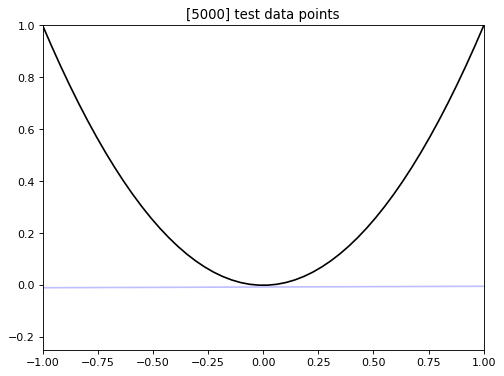
\includegraphics[width=0.75\linewidth]{png/single_exp_5k_5k.png}\end{center}
        
        \pagebreak
        
        \item Running these trials showed that the main indicator of result quality was, obviously, the number of training sets.  With less than a hundred sets the average function, $\Bias$, and $\Var$ varied wildly.  Around a thousand sets it stabilized significantly near the numbers reported in (a) above.
        This is easily seen in the following plots.  The results for each of the three runs (2500, 5000, and 10,000 test points) were not substantially different so only the plots for 5000 points are shown here.  The others are attached at the end.
        \\\\
        The first plot shows $\Bias$ as a blue dashed line, and $\Var$ as a red dotted line.  The second plot shows $\Expect[E_{test}] - (\Bias + \Var)$ (it is slightly mislabeled).  On the third plot, a shift in color from red to blue indicates increasing number of data sets used to generate the average function, hence the thick purple band centered near zero.  
        \begin{center}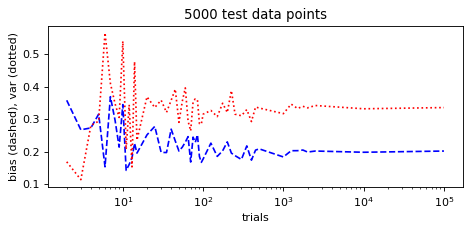
\includegraphics[width=0.9\linewidth]{png/5000_data_points_bias-var.png}\end{center}
        \begin{center}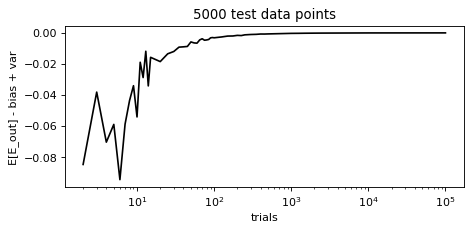
\includegraphics[width=0.9\linewidth]{png/5000_data_points_diff.png}\end{center}
\pagebreak
        \begin{center}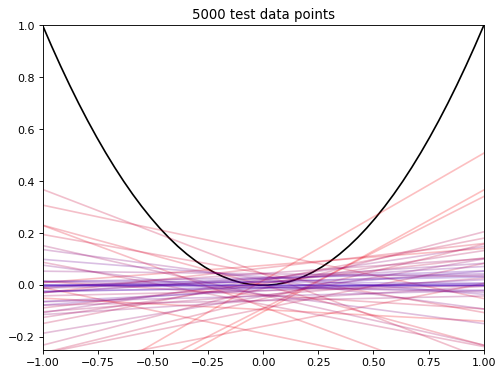
\includegraphics[width=0.75\linewidth]{png/5000_test_data_points.png}\end{center}
        \item Running these trials showed, unsurprisingly, that having a low number of trials (average functions) produced poor results.  This can be seen in part (b) as well, but is especially clear here.  I ran this part to see if there were any interesting trends in $\Bias$ and $\Var$.  $\Var$ was always greater than $\Bias$ and it's shape matched $\Bias$ more closely than in part (b).
        \\\\
        In the typical case, $\Bias$ and $\Var$ were more unstable than in part (b).  Interestingly, they stabilized around 1,000 test points.  In part (b) they stabilized around 1,000 trials (average functions).
        \begin{center}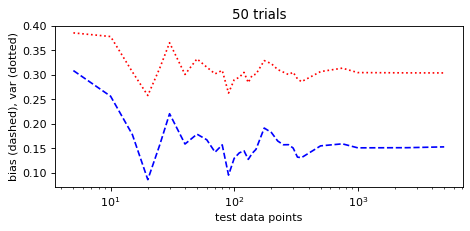
\includegraphics[width=0.9\linewidth]{png/50_trials_bias-var.png}\end{center}
\pagebreak
        \begin{center}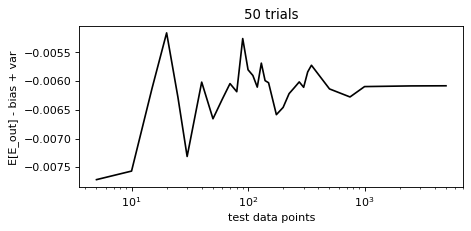
\includegraphics[width=0.9\linewidth]{png/50_trials_diff.png}\end{center}
        \begin{center}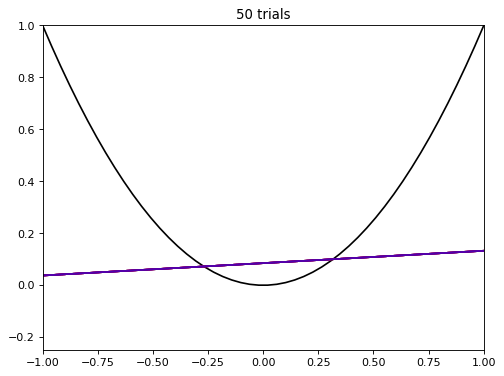
\includegraphics[width=0.75\linewidth]{png/50_trials.png}\end{center}
    \end{enumerate}
\pagebreak
    \item Analytic Solutions
    \begin{enumerate}
        \item The value of $\Bias$ is:
            \begin{equation*}
                \Expect_{x}[\Bias(x)] = \int_{x} (\bar{g}(x) - x^{2})^{2}\frac{1}{2}dx 
                = \int_{x} (- x^{2})^{2}\frac{1}{2}dx = \frac{1}{2}\int_{-1}^{1} x^{4}dx
                = \frac{1}{2}\frac{x^{5}}{5}\Biggr|^{1}_{-1}
                =\frac{1}{5}
            \end{equation*}
        
        \item The value of $\Var$ is:
        
    \begin{align*}
    \Var &= \Expect_{x}\Expect_{\Data}[(g^{\Data}(x) - \bar{g}(x))^{2}]
        =\Expect_{\Data}\Expect_{x}[g^{\Data}(x)]
        = \Expect_{\Data}\Expect_{x}[(x_{2}x + x_{1}x - x_{2}x_{1})^{2}]\\
        &=
        \Expect_{\Data}\Expect_{x}[x_{1}^{2}x^{2}]
        +\Expect_{\Data}\Expect_{x}[x_{2}^{2}x^{2}]\\
        &\quad \quad \quad
        -2\Expect_{\Data}[x_{1}^{2}x_{2}]\Expect_{x}[x]
        -2\Expect_{\Data}[x_{1}x_{2}^{2}]\Expect_{x}[x]
        +\Expect_{\Data}\Expect_{x}[x_{1}x_{2}x^{2}]
        \\
        &=
        \Expect_{\Data}\Expect_{x}[x_{1}^{2}x^{2}]
        +\Expect_{\Data}\Expect_{x}[x_{2}^{2}x^{2}]
        +\Expect_{\Data}\Expect_{x}[x_{1}^{2}x_{2}^{2}]\\
        &\quad \quad \quad 
        -2\Expect_{\Data}\Expect_{x}[x_{1}^{2}x_{2}x]
        -2\Expect_{\Data}[x_{1}x_{2}^{2}]\Expect_{x}[x]
        +\Expect_{x_{2}}\Expect_{x}[\Expect_{x_{1}}[x_{1}]]\\
        &=
        \Expect_{\Data}\Expect_{x}[x_{1}^{2}x^{2}]
        +\Expect_{\Data}\Expect_{x}[x_{2}^{2}x^{2}]\\
        &=
        \Expect_{x_{1}}[x_{1}^{2}]\Expect_{x}[x^{2}]
        +
        \Expect_{x_{2}}[x_{2}^{2}]\Expect_{x}[x^{2}]
        +
        \Expect_{x_{1}}[x_{1}^{2}]\Expect_{x_{2}}[x_{2}^{2}]\\
        &=
        \frac{1}{9}
        +
        \frac{1}{9}
        +
        \frac{1}{9}\\
        &= \frac{1}{3}
    \end{align*}
    Because $\Expect_{u}[u] = 0$ and $\Expect_{u}[u^2] = \frac{1}{9}$ when $u$ is uniformly distributed over $[-1, 1]$.
            
        \item The expected out of sample error is:
            \begin{equation*}
               \Expect[\ErrOut] = \Bias + \Var = \frac{8}{15}
            \end{equation*}
    \end{enumerate}
\end{enumerate}

\pagebreak

\section*{Problem 2.22}
\begin{enumerate}
\item Show that if $y(\X) = f(\X) + \epsilon$, where $\epsilon$ is a zero-mean noise random variable with variance $\sigma^{2}$, then the bias-variance decomposition becomes $\Expect_{\Data}[\ErrOut(\gD] = \sigma^{2} + \Bias + \Var$.
% \begin{equation*}
%     \Expect_{\Data}[\ErrOut(\gD] = \sigma^{2} + \Bias + \Var
% \end{equation*}
\begin{align*}
    \Expect_{\Data}[\ErrOut(\gD] 
    &= \Expect_{\Data}
    [ 
        \Expect_{\X,y} [(y(\X) - \gD(\X))^{2}]
    ]
    \\
    &= \Expect_{\Data} [\Expect_{\X,\epsilon}[(f(\X) + \epsilon - \gD(\X))^{2}] ]
    \\
    &= \Expect_{x,\Data} [\Expect_{\epsilon} [(f(\X) + \epsilon - \gD(\X))^{2}]]
    \\
    &= \Expect_{x,\Data} 
    [
    \Expect_{\epsilon}
    [
        f(\X)^{2} + \epsilon^{2} + \gD(\X)^{2} + 2\epsilon f(\X) + 2\epsilon\gD(\X) - 2f(\X)\gD(\X)
    ] 
    ]
    \\
    &= \Expect_{x,\Data} 
    [
    \Expect_{\epsilon}
    [
        f(\X)^{2} + \epsilon^{2} + \gD(\X)^{2} - 2f(\X)\gD(\X)]
            + \underbrace{\Expect_{\epsilon}[2\epsilon f(\X)]}_{0}
            - \underbrace{\Expect_{\epsilon}[2\epsilon\gD(\X)]}_{0}
    ]
    \\
    &= \Expect_{x,\Data} 
    [
    \underbrace{\Expect_{\epsilon}[f(\X)^{2}]}
    _{f(\X)^{2}}
    +
    \underbrace{\Expect_{\epsilon}[\epsilon^{2}]}
    _{\Var(\epsilon) + \Expect_{\epsilon}[\epsilon]}
    +
    \underbrace{\Expect_{\epsilon}[\gD(\X)^{2}]}
    _{\gD(\X)^{2}}
    -
    \underbrace{\Expect_{\epsilon}[2f(\X)\gD(\X)]}
    _{2f(\X)\gD(\X)}
    ]
    \\
    &= \Expect_{x}\Expect_{\Data}
    [
        f(\X)^{2} + 
        \bigl(
        \,
        \underbrace{\Var(\epsilon)}_{\sigma^{2}}
        + 
        \underbrace{\Expect_{\epsilon}[\epsilon]}_{0}
        \,
        \bigr)
        + \gD(\X)^{2} - 2 f(\X)\gD(\X)
    ]
    \\
    &= \Expect_{x}\Expect_{\Data}
    [
        f(\X)^{2} + \sigma^{2} + \gD(\X)^{2} - 2 f(\X)\gD(\X)
    ]    
    \\
    &= \Expect_{\X}
    [
    \underbrace{\Expect_{\Data}[f(\X)^{2}]}_{f(\X)^{2}}
    +
    \underbrace{\Expect_{\Data}[\sigma^{2}]}_{\sigma^{2}}
    +
    \underbrace{\Expect_{\Data}[\gD(\X)^{2}]}
    _{\substack{\Var_{\Data}[\gD(\X)] \\[0.5ex] + \\[0.5ex] \Expect_{\Data}[\gD(\X)]^{2}}}
    -
        \underbrace{\Expect_{\Data}[2f(\X)]}_{2f(\X)}
            \cdot
        \Expect_{\Data}[\gD(\X)]
    ]
    \\
    &= \Expect_{\X}
    [
    \sigma^{2} + \Var_{\Data}[\gD(\X)]
    + f(\X)^{2} - 2f(\X)\underbrace{\Expect_{\Data}[\gD(\X)]}_{\bar{g}(\X)} + \underbrace{\Expect_{\Data}[\gD(\X)]^{2}}_{\bar{g}(\X)^{2}}
    ]
    \\
    &= \Expect_{\X}
    [
    \sigma^{2} + \underbrace{\Var_{\Data}[\gD(\X)]}_{\Var(\X)}
    + 
    \underbrace
    {f(\X)^{2} - 2f(\X)\bar{g}(\X) + \bar{g}(\X)^{2}}
    _{( f(\X) - \bar{g}(\X))^{2}}
    ]
    \\
    &= \Expect_{\X}
    [
    \sigma^{2} + \Var(\X) + (f(\X) - \bar{g}(\X))^{2}
    ]
    \\
    &=
    \underbrace
    {\Expect_{\X}[\sigma^{2}]}_{\sigma^{2}}
    +
    \underbrace
    {\Expect_{\X}[\Var(\X)]}_{\Var}
    + 
    \underbrace
    {\Expect_{\X}[(f(\X) - \bar{g}(\X))^{2}]}_{\Bias}
    \\
    &= \sigma^{2} + \Bias + \Var
\end{align*}
Because $\Expect_{\epsilon}[\epsilon] = 0$ (since it has zero-mean) and $\Expect_{u}[f] = f$ when $f$ does not depend on $u$.
\end{enumerate}

\pagebreak
\section*{All code}
\lstset{style=mystyle_top}
\begin{lstlisting}[language=Python, caption=experiement\_funcs.py]
import numpy as np
from numpy.random import default_rng
import warnings

# ############## DEFINE EXPERIMENT ############### DEFINE EXPERIMENT ############### DEFINE EXPERIMENT ############## #
# Seed a rng so all test sets have the same sequence, for result comparability.
test_set_rng = default_rng(0)

# Configure exception handling for testing
overflow_err_state = "raise"
max_attempts = 15


# This is a top-level experiment function.  Do a number of experiments of varying trial counts
def doExperimentSetTrials(trial_count_set, test_size):
    sz_list = []
    hyp_list = []
    stat_list = []
    for trial_count in trial_count_set:
        test_data = test_set_rng.uniform(-1, 1, test_size)

        for attempt in range(0, max_attempts):
            try:
                hypothesis_set = findHypothesisSet(trial_count)
                experiment_results = calcExperimentOutputs(test_data, hypothesis_set)
            except FloatingPointError:
                if attempt == max_attempts - 1:
                    print("Attempt ", attempt + 1, " failed, aborting trial count: ", trial_count)
                    break
                else:
                    print("Caught in doExperimentSetTrials, retrying with attempt:", attempt + 2, " of ", max_attempts)
            else:
                exp_size = np.array([trial_count, test_size])

                sz_list.append(exp_size)
                hyp_list.append(experiment_results[0])
                stat_list.append(experiment_results[1])
                break

    return np.array(sz_list), np.array(hyp_list), np.array(stat_list)


# This is a top-level experiment function.  Do a number of experiments of varying test data sizes
def doExperimentSetTests(trial_count, test_sizes_set):
    sz_list = []
    hyp_list = []
    stat_list =[]
    hypothesis_set = findHypothesisSet(trial_count)
    for test_size in test_sizes_set:
        for attempt in range(0, max_attempts):
            try:
                test_data = test_set_rng.uniform(-1, 1, test_size)
                experiment_results = calcExperimentOutputs(test_data, hypothesis_set)
            except FloatingPointError:
                if attempt == max_attempts - 1:
                    print("Attempt ", attempt + 1, " failed, aborting test size: ", test_size)
                    break
                else:
                    print("Caught in deExperimentSetTests, retrying with attempt:", attempt + 2, " of ", max_attempts)
            else:
                exp_size = np.array([trial_count, test_size])

                sz_list.append(exp_size)
                hyp_list.append(experiment_results[0])
                stat_list.append(experiment_results[1])
                break
    return np.array(sz_list), np.array(hyp_list), np.array(stat_list)


# Given a number of trials t, generate t training-sets and find the hypothesis for each one
def findHypothesisSet(trials):
    hypothesis_set = np.empty((trials, 2))
    for i in range(0, trials - 1):
        data_set = getDataSet()
        hypothesis_set[i] = getHypothesis(data_set)

    return hypothesis_set


# Given a list of hypotheses, get the average function, bias, var, and two versions of E[E_out]
def calcExperimentOutputs(x_values, hypothesis_set):
    averageHypothesis = findExpectedHypothesis(hypothesis_set)
    try:
        bias = getBias(x_values, averageHypothesis)
        var = getVar(x_values, hypothesis_set, averageHypothesis)
        EEout = getEEout(x_values, hypothesis_set)
    except FloatingPointError:
        print("Caught exception in calcExperimentOutputs")
        raise FloatingPointError

    return averageHypothesis, np.array([bias, var, EEout])


# ############ GET EXPERIMENT INPUT ############ GET EXPERIMENT INPUT ############# GET EXPERIMENT INPUT ############ #


# Get data set
def getDataSet():
    x_one = np.random.uniform(-1, 1)
    x_two = np.random.uniform(-1, 1)
    return np.array([[x_one, x_one ** 2], [x_two, x_two ** 2]])


# ############## CALCULATION FUNCS ############### CALCULATION FUNCS ############### CALCULATION FUNCS ############## #


# Get the hypothesis:
def getHypothesis(data_set):
    return data_set[1][0] + data_set[0][0], -(data_set[0][0]*data_set[1][0])


# Return the average function, the mean of many hypotheses
def findExpectedHypothesis(manyTrialsResults):
    return np.mean(manyTrialsResults, 0)


# Evaluate a g(x) = ax + b at x
def evaluateLineAtX(x, coefficients):
    return coefficients[0] * x + coefficients[1]


# Take the bias over a new data set
def getBias(x_values, averageFunction):
    evaluation = evaluateLineAtX(x_values, averageFunction)
    with np.errstate(over=overflow_err_state):
        try:
            deviation = evaluation - np.square(x_values)
            bias = np.mean(np.square(deviation))
        except FloatingPointError:
            print("Catching overflow in getBias")
            raise FloatingPointError
    return bias


# Find the sample variance over test data
def getVar(x_values, hypothesis_set, averageFunction):
    num_hyps = len(hypothesis_set)
    deviation = hypothesis_set - averageFunction
    error_matrix = np.tensordot(deviation[:, 0], x_values, 0) + deviation[:, 1:]
    with np.errstate(over=overflow_err_state):
        try:
            error_matrix = np.square(error_matrix)
        except FloatingPointError:
            print("Catching overflow in getVar")
    mean_over_x = np.mean(error_matrix, 1)
    return np.sum(mean_over_x) / (num_hyps - 1)


# E[E_out] as mean approximation of expectation over data sets and test data
def getEEout(x_values, hypothesis_set):
    evaluation = np.tensordot(hypothesis_set[:, 0], x_values, 0) + hypothesis_set[:, 1:]
    with np.errstate(over=overflow_err_state):
        try:
            deviation = evaluation - np.square(x_values)
            error_matrix = np.square(deviation)
        except FloatingPointError:
            print("Catching overflow in getEEout")
    return np.mean(error_matrix)
\end{lstlisting}

\begin{lstlisting}[language=Python, caption=experiment\_printer.py]
import matplotlib.pyplot as plt
import numpy as np
import experiment_funcs as expf


def resultPrinterGeneral(result_row, filename):

    num_trials = result_row[0][0]
    test_size = result_row[0][1]
    avg_func = getLineEquationAsString(result_row[1])
    bias = result_row[2][0]
    var = result_row[2][1]
    eeout = result_row[2][2]

    print("# of Trials: ", num_trials, "; test data set size: ", test_size, file=filename)
    print("-------------------------------------------------------------", file=filename)
    print("g_hat(x)  = ", avg_func, file=filename)
    print("bias      = ", bias, file=filename)
    print("var       = ", var, file=filename)
    print("E[E_out]  = ", eeout, file=filename)
    print("", file=filename)
    print("bias + var = ", bias + var, file=filename)
    print("E[E_out] - (bias + var) = ", eeout - bias - var, file=filename)
    print("", file=filename)


def printLineEquation(coefficients, filename):
    print(coefficients[0], "x + ", coefficients[1], file=filename)


def getLineEquationAsString(coefficients):
    return "%sx + %s" % tuple(coefficients)


output_prefix = "results/final/"


def plotQuestionAnswer(results, title):
    fig, ax = plt.subplots()
    ax.set_title(title)
    ax.set_xlim(-1, 1)
    ax.set_ylim(-0.25, 1)
    target_x_range = np.linspace(-1, 1)
    target_y = np.square(target_x_range)
    ax.plot(target_x_range, target_y, c='k')

    num_hyps = len(results[1])
    alpha_bias = 0.75
    hyp_alpha = alpha_bias/num_hyps
    hyp_col_bias = 1
    hyp_col_shift = hyp_col_bias/num_hyps
    for hyp in results[1]:
        hyp_y = expf.evaluateLineAtX(target_x_range, hyp)
        hyp_alpha = 0.25
        ax.plot(target_x_range, hyp_y, alpha=hyp_alpha, c=(1 - hyp_col_shift, 0, hyp_col_shift))
        if hyp_alpha >= 1:
            hyp_alpha = 1
        else:
            hyp_alpha += alpha_bias/num_hyps
        if hyp_col_shift >= 1:
            hyp_col_shift = 1
        else:
            hyp_col_shift += alpha_bias/num_hyps

    fig.show()
    fig.savefig(output_prefix + title + '.png', transparent=False, dpi=80, bbox_inches="tight")
    plt.close(fig)


def initPlot_trials(sup_title, x_label, y_label, x_ticks, y_ticks, x_scale, y_scale):
    trials_fig, trials_ax = plt.subplots()
    trials_fig.set_size_inches(6, 3)

    super_title = sup_title
    trials_ax.set_title(sup_title)

    trials_ax.set_xlabel(x_label)
    trials_ax.set_ylabel(y_label)

    trials_ax.set_xscale(x_scale)
    trials_ax.set_yscale(y_scale)

    return trials_fig, trials_ax


def trials_plotter(results):

    # print(results)
    title = str(results[0][0][1]) + " test data points"
    file_title = str(results[0][0][1]) + "_data_points"
    x_trials_range = results[0][:, 0]
    y_bias_range = results[2][:, 0]
    y_var_range = results[2][:, 1]
    y_ticks = np.concatenate((results[2][:, 0], results[2][:, 1]))
    fig_bias_var, ax_bias_var = initPlot_trials(title, "trials", "bias (dashed), var (dotted)", x_trials_range, y_ticks, "log", "linear")

    ax_bias_var.plot(x_trials_range, y_bias_range, ls='dashed', c='b')
    ax_bias_var.plot(x_trials_range, y_var_range, ls='dotted', c='r')

    fig_bias_var.show()
    fig_bias_var.savefig(output_prefix + file_title + '_bias-var' + '.png', transparent=False, dpi=80, bbox_inches="tight")
    plt.close(fig_bias_var)

    # #########

    y_bias_var_range = y_bias_range + y_var_range
    y_eeout_range = results[2][:, 2]

    y_diff_range = y_eeout_range - y_bias_var_range
    fig_bias_var_diff, ax_bias_var_diff = initPlot_trials(title, "trials", "E[E_out] - bias + var ", x_trials_range, y_diff_range, "log", "linear")

    ax_bias_var_diff.plot(x_trials_range, y_diff_range, c='k')

    fig_bias_var_diff.show()
    fig_bias_var_diff.savefig(output_prefix + file_title + '_diff' + '.png', transparent=False, dpi=80, bbox_inches="tight")
    plt.close(fig_bias_var_diff)


def tests_plotter(results):

    # print(results)
    title = str(results[0][0][0]) + " trials"
    file_title = str(results[0][0][0]) + "_trials"
    x_trials_range = results[0][:, 1]
    y_bias_range = results[2][:, 0]
    y_var_range = results[2][:, 1]
    y_ticks = np.concatenate((results[2][:, 0], results[2][:, 1]))
    fig_bias_var, ax_bias_var = initPlot_trials(title, "test data points", "bias (dashed), var (dotted)", x_trials_range, y_ticks, "log", "linear")

    # ax_bias_var.set_yscale("symlog", linthresh=.0000000000000001)
    ax_bias_var.plot(x_trials_range, y_bias_range, ls='dashed', c='b')
    ax_bias_var.plot(x_trials_range, y_var_range, ls='dotted', c='r')
    fig_bias_var.show()
    fig_bias_var.savefig(output_prefix + file_title + '_bias-var' + '.png', transparent=False, dpi=80, bbox_inches="tight")
    plt.close(fig_bias_var)

    # #########

    y_bias_var_range = y_bias_range + y_var_range
    y_eeout_range = results[2][:, 2]

    y_diff_range = y_eeout_range - y_bias_var_range
    fig_bias_var_diff, ax_bias_var_diff = initPlot_trials(title, "test data points", "E[E_out] - bias + var ", x_trials_range, y_diff_range, "log", "linear")

    ax_bias_var_diff.plot(x_trials_range, y_diff_range, c='k')

    fig_bias_var_diff.show()
    fig_bias_var_diff.savefig(output_prefix + file_title + '_diff' + '.png', transparent=False, dpi=80, bbox_inches="tight")
    plt.close(fig_bias_var_diff)
    
\end{lstlisting}

\begin{lstlisting}[language=Python, caption=new\_meta\_experiment.py, captionpos=t]
import experiment_funcs as expf
import experiment_printer as expp
import numpy as np
import matplotlib.pyplot as plt


# ############## DO THE EXPERIMENT ############### DO THE EXPERIMENT ############### DO THE EXPERIMENT ############## #
seq_tiny = (2, 3, 4, 5)
seq_small = (5, 10, 25, 50, 100)
seq_medium = (10, 25, 75, 150, 500)
seq_big = (10, 15, 20, 25, 50, 75, 100, 150, 175, 200, 250, 500, 1000)
seq_massive = (10, 100, 1000, 10000, 100000, 1000000, 10000000)


# Final sequence to use for both varying trial count, and varying test size
final_trial_count_seq = (2, 3, 4, 5, 6, 7, 8, 9, 10, 11, 12, 13, 14, 15, 20, 25, 30, 35, 40, 45, 50, 55, 60, 65, 70, 75, 80, 85, 90, 95, 100, 125, 150, 175, 200, 225, 250, 300, 350, 400, 450, 500, 1000, 1250, 1500, 1750, 2000, 2500, 10000, 100000)
final_test_count_seq = (5, 10, 15, 20, 25, 30, 40, 50, 60, 70, 80, 90, 100, 110, 120, 130, 140, 150, 175, 200, 225, 250, 275, 300, 325, 350, 500, 750, 1000, 2500, 5000)

# Alias this so as to not change following code during program debug/testing.
alias_trial_count_seq = final_trial_count_seq
alias_test_count_seq = final_test_count_seq


# Generate results for reports, varying number of trials on fixed test size
def metaExperiment_trials(trial_count_set, test_size, output_file):
    print("======== DOING TRIALS (", trial_count_set[0], ", ..., ", trial_count_set[-1],
          ") with ", test_size, " test points ========", file=output_file)
    results = expf.doExperimentSetTrials(trial_count_set, test_size)

    for i in range(0, len(results[0])):
        result_row = results[0][i], results[1][i], results[2][i]
        expp.resultPrinterGeneral(result_row, output_file)

    expp.trials_plotter(results)
    expp.plotQuestionAnswer(results, str(results[0][0][1]) + " test data points")


# Generate results for reports, varying number of tests on fixed trial size
def metaExperiment_tests(trial_count, test_data_sizes, output_file):
    print("======== DOING TESTS (", test_data_sizes[0], ", ..., ", test_data_sizes[-1],
          ") with ", trial_count, " trial size ========", file=output_file)
    results = expf.doExperimentSetTests(trial_count, test_data_sizes)

    for i in range(0, len(results[0])):
        result_row = results[0][i], results[1][i], results[2][i]
        expp.resultPrinterGeneral(result_row, output_file)

    expp.tests_plotter(results)
    expp.plotQuestionAnswer(results, str(results[0][0][0]) + " trials")


# ############## DO THE EXPERIMENT ############### DO THE EXPERIMENT ############### DO THE EXPERIMENT ############## #
# In every innermost function call, test data is generated by a seeded generator, so the sequence is fixed
# In every innermost function call, training data is generated by an un-seeded generator, so the sequence is different

# In this section metaExperiment_trials increments trial count
output_prefix = "results/final/"
print("Doing 2500 test data")
results_2500_test = open(output_prefix + "results_test_points_2500.dat", 'w')
metaExperiment_trials(alias_trial_count_seq, 2500, results_2500_test)
results_2500_test.close()
# # # ################
print("Doing 5000 test")
results_5000_test = open(output_prefix + "results_test_points_5000.dat", 'w')
metaExperiment_trials(alias_trial_count_seq, 5000, results_5000_test)
results_5000_test.close()
# # # ################
print("Doing 10000 test data")
results_10000_test = open(output_prefix + "results_test_points_10000.dat", 'w')
metaExperiment_trials(alias_trial_count_seq, 10000, results_10000_test)
results_10000_test.close()
# # # ################
# # # ################

# # In this section metaExperiment_tests increments test data size
print("Doing 25 trials")
results_25_trials = open(output_prefix + "results_trials_25.dat", 'w')
metaExperiment_tests(25, alias_trial_count_seq, results_25_trials)
results_25_trials.close()
# # ################
print("Doing 50 trials")
results_50_trials = open(output_prefix + "results_trials_50.dat", 'w')
metaExperiment_tests(50, alias_trial_count_seq, results_50_trials)
results_50_trials.close()
# # # ################
print("Doing 100 trials")
results_100_trials = open(output_prefix + "results_trials_100.dat", 'w')
metaExperiment_tests(100, alias_trial_count_seq, results_100_trials)
results_100_trials.close()
# # # ################
single_name = "results/final/single_exp_5000_5000.dat"
single_file = open(single_name, "w")
metaExperiment_trials(np.array([5000]), np.array([5000]), single_file)
single_file.close()

# ##########################################
print("All done!")
\end{lstlisting}
%%%%%%%%%%%%%%%%%%
\pagebreak
\section*{All data and plots}
This is the single experiment shown in part (a):
\VerbatimInput[label=\fbox{\color{Black}single\_exp\_5000\_5000.dat}]{dat/single_exp_5000_5000.dat}
        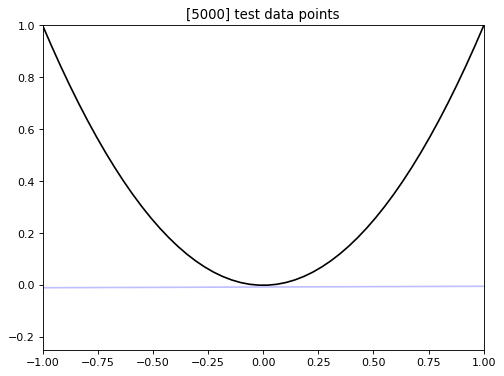
\includegraphics[width=0.9\linewidth]{png/single_exp_5k_5k.png}
 \\On the following pages are all data and plots for the other experiments.
\pagebreak
\VerbatimInput[label=\fbox{\color{Black}results\_test\_points\_2500.dat}]{dat/results_test_points_2500.dat}
\pagebreak
        \begin{center}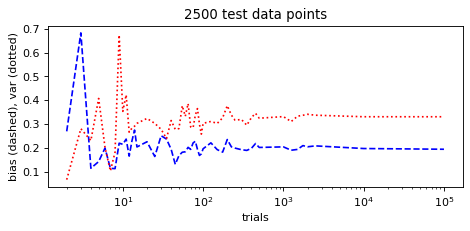
\includegraphics[width=0.7\linewidth]{png/2500_data_points_bias-var.png}\end{center}
        \begin{center}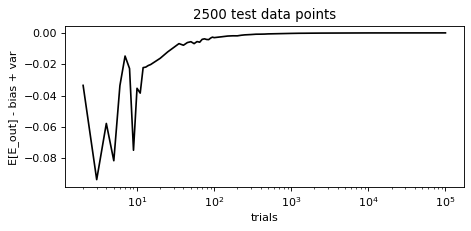
\includegraphics[width=0.7\linewidth]{png/2500_data_points_diff.png}\end{center}
        \begin{center}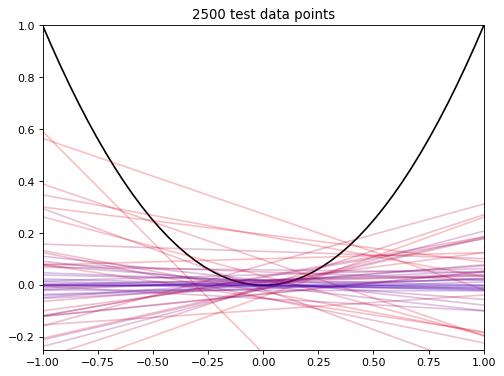
\includegraphics[width=0.68\linewidth]{png/2500_test_data_points.png}\end{center}

\pagebreak        
\VerbatimInput[label=\fbox{\color{Black}results\_test\_points\_5000.dat}]{dat/results_test_points_5000.dat}
\pagebreak
        \begin{center}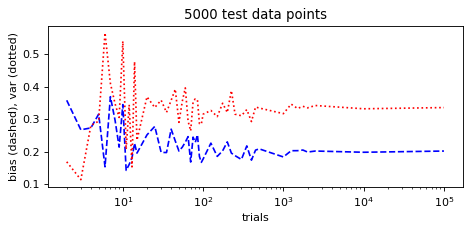
\includegraphics[width=0.7\linewidth]{png/5000_data_points_bias-var.png}\end{center}
        \begin{center}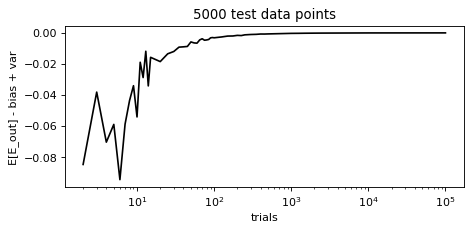
\includegraphics[width=0.7\linewidth]{png/5000_data_points_diff.png}\end{center}
        \begin{center}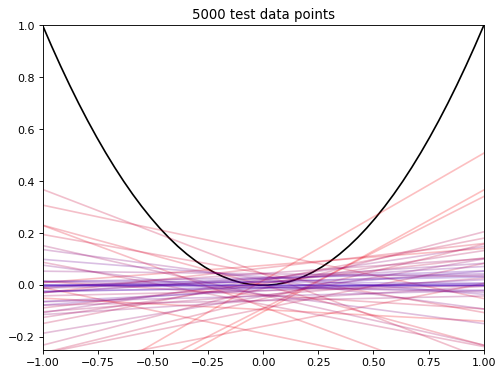
\includegraphics[width=0.68\linewidth]{png/5000_test_data_points.png}\end{center}

\pagebreak        
\VerbatimInput[label=\fbox{\color{Black}results\_test\_points\_10000.dat}]{dat/results_test_points_10000.dat}
\pagebreak
        \begin{center}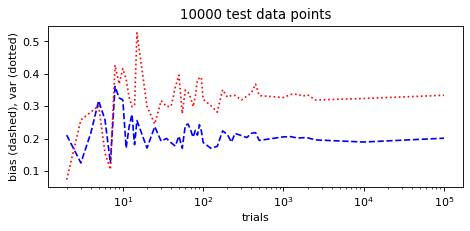
\includegraphics[width=0.7\linewidth]{png/10000_data_points_bias-var.png}\end{center}
        \begin{center}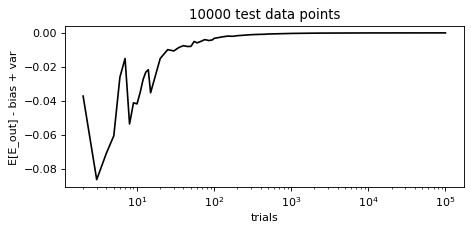
\includegraphics[width=0.7\linewidth]{png/10000_data_points_diff.png}\end{center}
        \begin{center}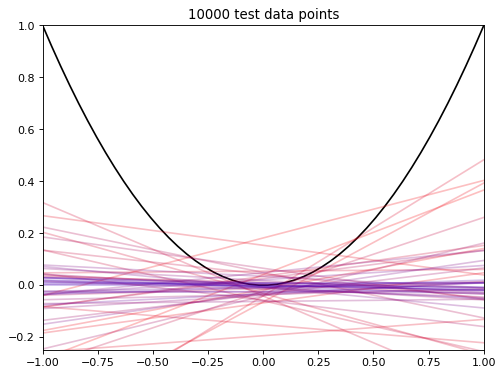
\includegraphics[width=0.68\linewidth]{png/10000_test_data_points.png}\end{center}

\pagebreak   
\VerbatimInput[label=\fbox{\color{Black}results\_trial2\_25.dat}]{dat/results_trials_25.dat}
% \pagebreak
        \begin{center}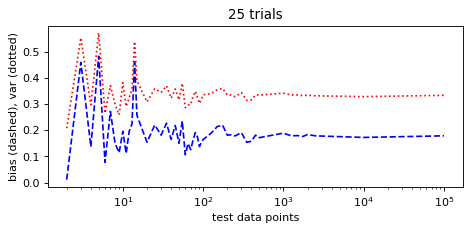
\includegraphics[width=0.6\linewidth]{png/25_trials_bias-var.png}\end{center}
        \begin{center}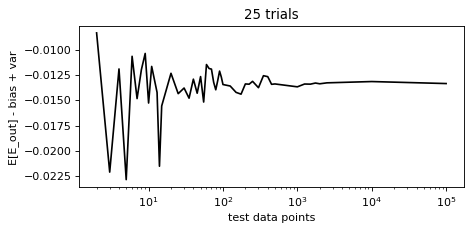
\includegraphics[width=0.6\linewidth]{png/25_trials_diff.png}\end{center}
        \begin{center}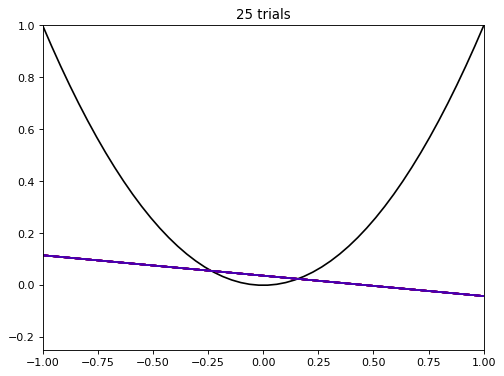
\includegraphics[width=0.58\linewidth]{png/25_trials.png}\end{center}
        
\pagebreak        
\VerbatimInput[label=\fbox{\color{Black}results\_pathological\_50.dat}]{dat/results_trials_50.dat}
% \pagebreak
        \begin{center}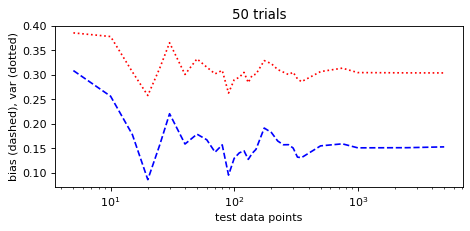
\includegraphics[width=0.6\linewidth]{png/50_trials_bias-var.png}\end{center}
        \begin{center}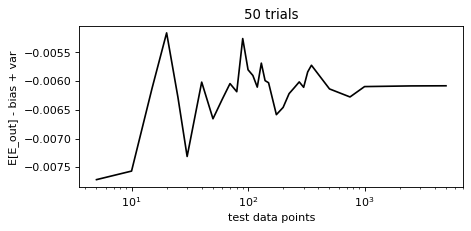
\includegraphics[width=0.6\linewidth]{png/50_trials_diff.png}\end{center}
        \begin{center}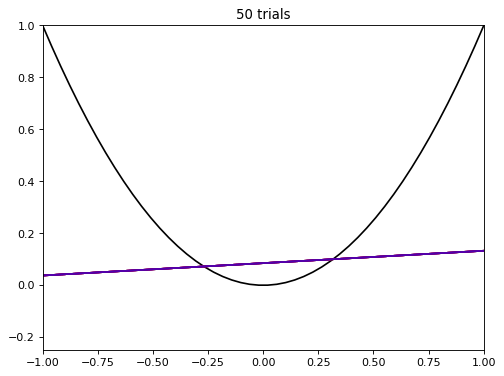
\includegraphics[width=0.58\linewidth]{png/50_trials.png}\end{center}
        
\pagebreak
\VerbatimInput[label=\fbox{\color{Black}results\_trial2\_100.dat}]{dat/results_trials_100.dat}
% \pagebreak
        \begin{center}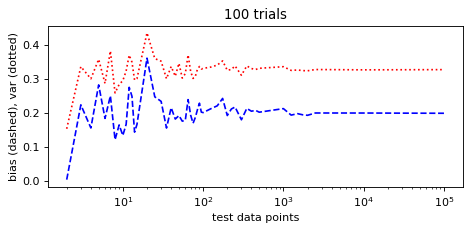
\includegraphics[width=0.6\textwidth]{png/100_trials_bias-var.png}\end{center}
        \begin{center}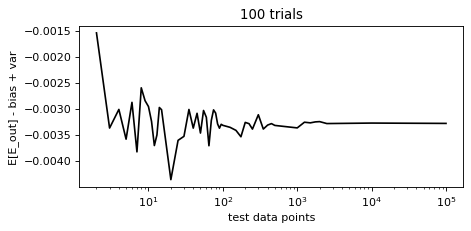
\includegraphics[width=0.6\textwidth]{png/100_trials_diff.png}\end{center}
        \begin{center}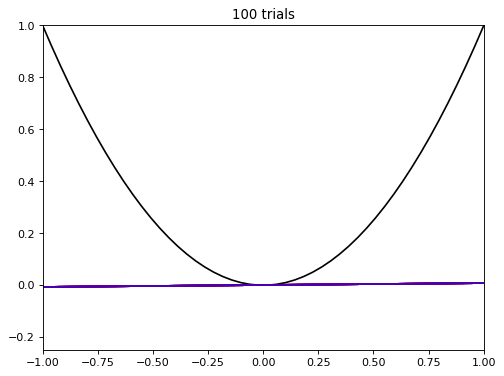
\includegraphics[width=0.58\linewidth]{png/100_trials.png}\end{center}

\printbibliography[title={AML Book}]
\end{document}